\subsection{Verifizierung des Funktionsweise des Lock-In-Verstärkers}
Die Spannungen werden für die Phasenverschiebungen $\varphi= \SI{0}{°}, \SI{90}{°}, \SI{180}{°}, \SI{270}{°}, \SI{315}{°}$ gespeichert und in Abbildung \ref{fig:0gradnormal},
Abbildung \ref{fig:90gradnormal}, Abbildung \ref{fig:180gradnormal}, Abbildung \ref{fig:270gradnormal} und Abbildung \ref{fig:315gradnormal} zu sehen.
\FloatBarrier
\begin{figure}[h!]
 \centering
 \begin{subfigure}{0.48\textwidth}
  \centering
  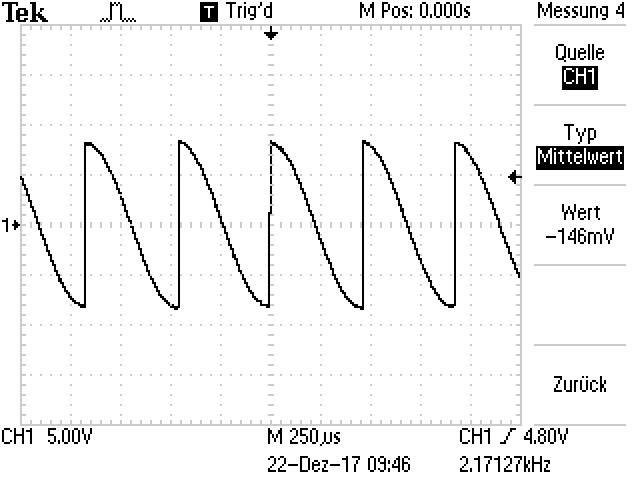
\includegraphics[width=\textwidth]{0gradnormal.JPG}
  \caption{Spannung bei $\varphi=\SI{0}{°}$}
  \label{fig:0gradnormal}
 \end{subfigure}
 \begin{subfigure}{0.48\textwidth}
  \centering
  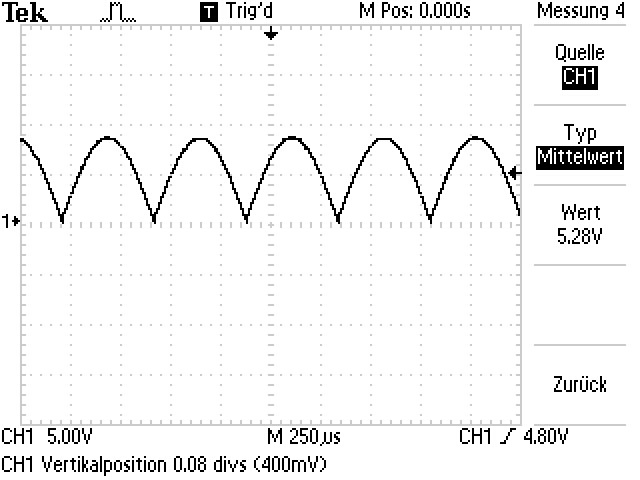
\includegraphics[width=\textwidth]{90gradnormal.JPG}
  \caption{Spannung bei $\varphi=\SI{90}{°}$}
  \label{fig:90gradnormal}
 \end{subfigure}
 \caption{Spannungsverläufe an dem Mischer}
 \label{fig:000090}
\end{figure}
\begin{figure}[h!]
 \centering
 \begin{subfigure}{0.48\textwidth}
  \centering
  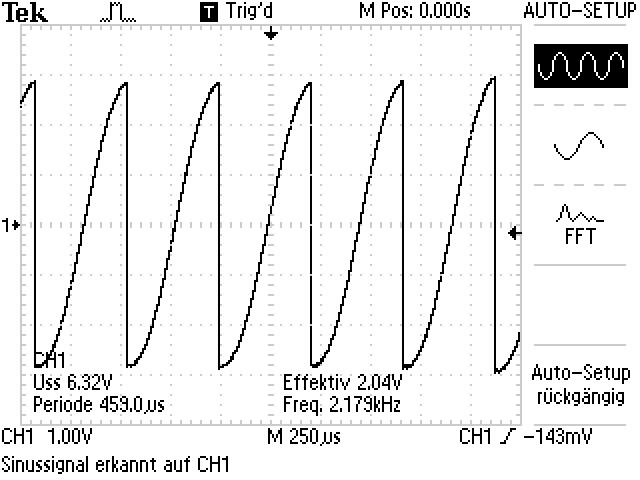
\includegraphics[width=\textwidth]{180gradnormal.JPG}
  \caption{Spannung bei $\varphi=\SI{180}{°}$}
  \label{fig:180gradnormal}
 \end{subfigure}
 \begin{subfigure}{0.48\textwidth}
  \centering
  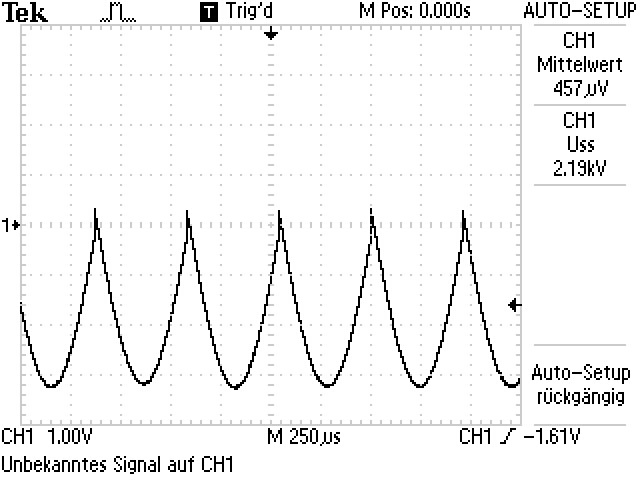
\includegraphics[width=\textwidth]{270gradnormal.JPG}
  \caption{Spannung bei $\varphi=\SI{270}{°}$}
  \label{fig:270gradnormal}
 \end{subfigure}
 \caption{Spannungsverläufe an dem Mischer}
 \label{fig:180270}
\end{figure}
\begin{figure}[h!]
  \centering
  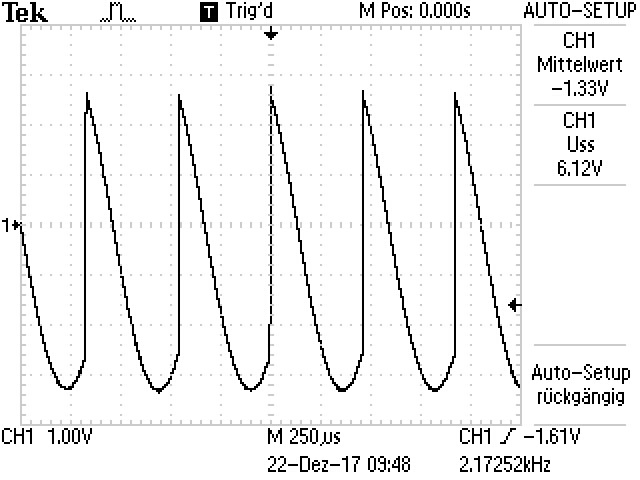
\includegraphics[width=0.48\textwidth]{315gradnormal.JPG}
  \caption{Spannung bei $\varphi=\SI{315}{°}$}
  \label{fig:315gradnormal}
\end{figure}
\FloatBarrier
Die Phasenverschiebung und die Amplitude sind in Tabelle \ref{tab:normal} aufgetragen.
\begin{table}[h!]
  \centering
  \caption{Erste Messreihe zur Verifizierung der Funktionsweise des Lock-In-Verstärkers}
  \label{tab:normal}
  \begin{tabular}{c c c}
    \toprule
     $\varphi/°$ & $\varphi/rad$ &	 A/V	   \\
    \midrule
    0   & 0,000  & -69,6  \\
    15  & 0,262	& -82,0  \\
    45  & 0,785	& -102,0 \\
    90  & 1,571	& -76,0  \\
    135 & 2,356	& -8,0   \\
    180 & 3,142	&  70,4  \\
    225 & 3,927	&  102,0 \\
    270 & 4,712	&  76,0  \\
    315 & 5,498	&  7,6   \\
    360 & 6,283	& -68,8  \\
    \bottomrule
  \end{tabular}
\end{table}

In Abbildung \ref{fig:refplot} ist die Phasenverschiebung $\varphi$ gegen die Spannungsamplitude $A$ aufgetragen.
\FloatBarrier
\begin{figure}[h!]
  \centering
  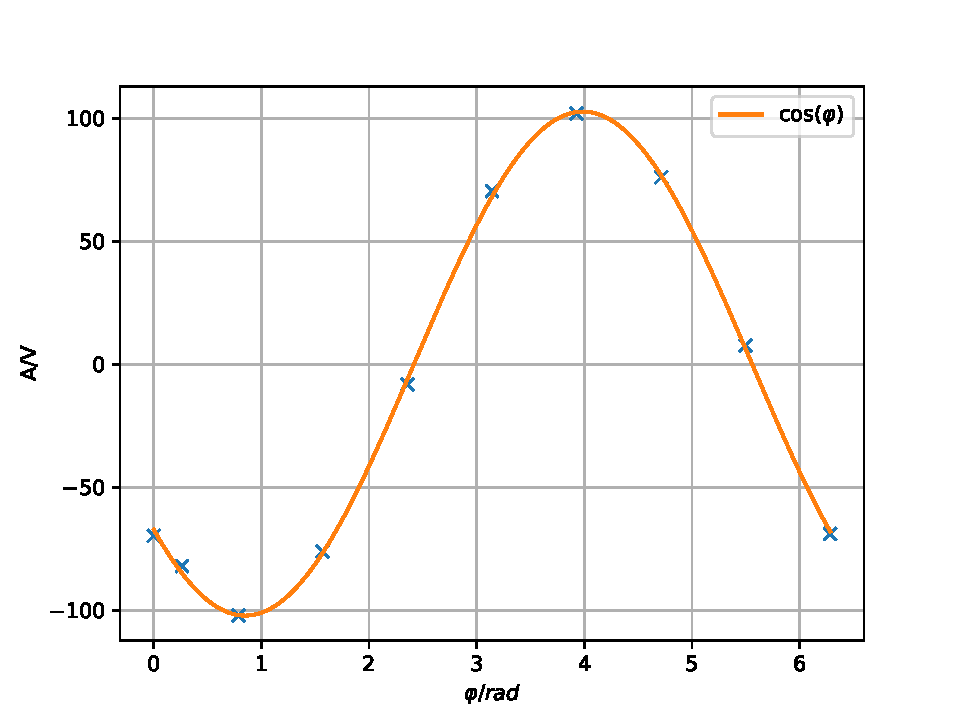
\includegraphics[width=\textwidth]{ref.pdf}
  \caption{Phasenverschiebung $\varphi$ gegen Spannungsamplitude $A$}
  \label{fig:refplot}
\end{figure}
\FloatBarrier
Gefittet ist eine $\cos$-Funktion nach Gleichung \eqref{eqn:uoutcos}:
\begin{equation*}
  A= a \cos{(bx+c)}+d.
\end{equation*}
Die Parameter ergeben sich mit Python 3.6.3 zu
\begin{align*}
  a &=& \SI{102.407   \pm 0.986}{V} \\
  b &=& \SI{  1.001   \pm 0.005}{}\\
  c &=& \SI{  2.291   \pm 0.018}{} \\
  d &=& \SI{  0.335   \pm 0.715}{V}  \\
\end{align*}
Da nach Gleichung \eqref{eqn:uoutcos} $a=\frac{2 \overline{U_{0}}}{\pi}$:
\begin{equation*}
  \overline{U_{0}}= \SI{160.861}{V}
\end{equation*}
\FloatBarrier
Die Spannungen bei den Phasenverschiebungen $\varphi= \SI{0}{°}, \SI{90}{°}, \SI{180}{°}, \SI{270}{°}, \SI{315}{°}$ mit eingeschaltetem Störgenerator sind in Abbildung \ref{fig:0gradrausch},
Abbildung \ref{fig:90gradrausch}, Abbildung \ref{fig:180gradrausch}, Abbildung \ref{fig:270gradrausch} und Abbildung \ref{fig:315gradrausch} dargestellt.
\FloatBarrier
\begin{figure}[h!]
 \centering
 \begin{subfigure}{0.48\textwidth}
  \centering
  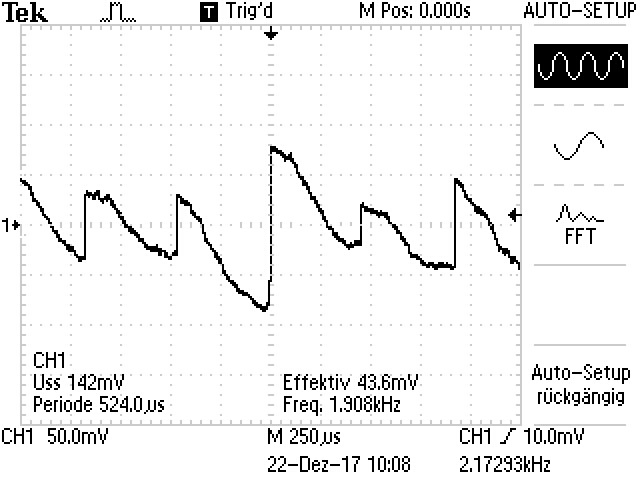
\includegraphics[width=\textwidth]{0gradrausch.JPG}
  \caption{Spannung bei $\varphi=\SI{0}{°}$ mit zugeschaltetem Rauschen}
  \label{fig:0gradrausch}
 \end{subfigure}
 \begin{subfigure}{0.48\textwidth}
  \centering
  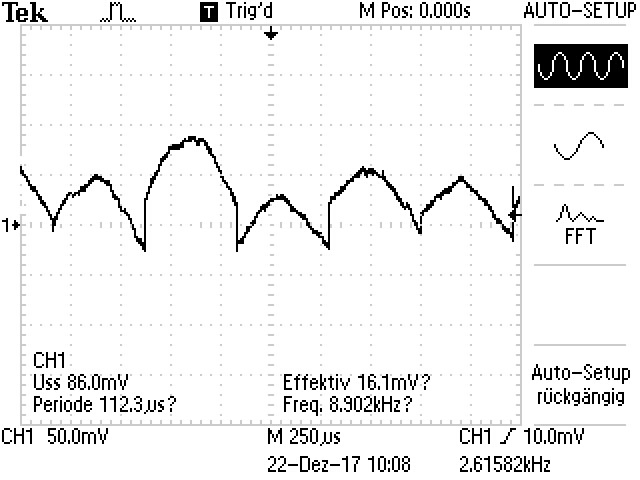
\includegraphics[width=\textwidth]{90gradrausch.JPG}
  \caption{Spannung bei $\varphi=\SI{90}{°}$ mit zugeschaltetem Rauschen}
  \label{fig:90gradrausch}
 \end{subfigure}
 \caption{Spannungsverläufe an dem Mischer}
 \label{fig:000090}
\end{figure}
\begin{figure}[h!]
 \centering
 \begin{subfigure}{0.48\textwidth}
  \centering
  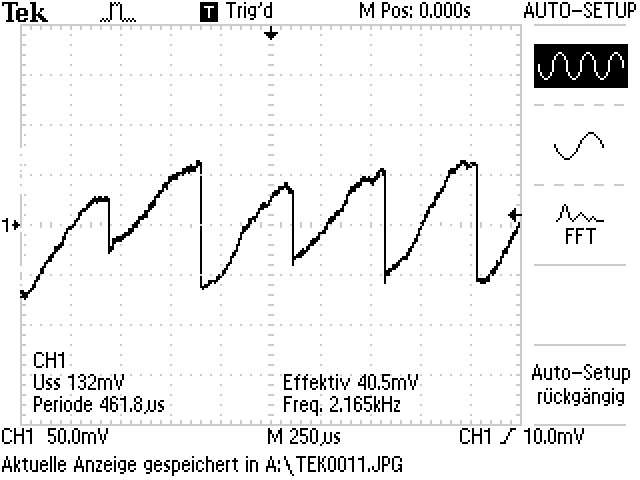
\includegraphics[width=\textwidth]{180gradrausch.JPG}
  \caption{Spannung bei $\varphi=\SI{180}{°}$ mit zugeschaltetem Rauschen}
  \label{fig:180gradrausch}
 \end{subfigure}
 \begin{subfigure}{0.48\textwidth}
  \centering
  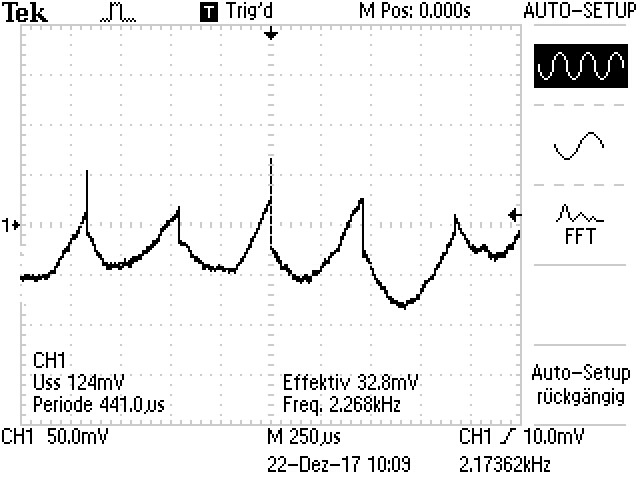
\includegraphics[width=\textwidth]{270gradrausch.JPG}
  \caption{Spannung bei $\varphi=\SI{270}{°}$ mit zugeschaltetem Rauschen}
  \label{fig:270gradrausch}
 \end{subfigure}
 \caption{Spannungsverläufe an dem Mischer}
 \label{fig:180270}
\end{figure}
\begin{figure}[h!]
  \centering
  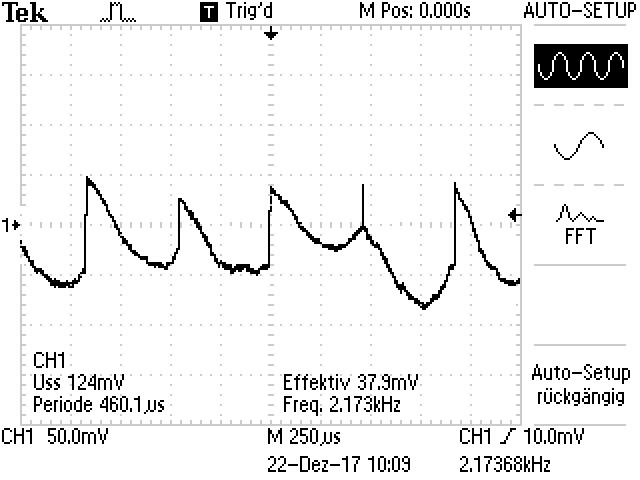
\includegraphics[width=0.48\textwidth]{315gradrausch.JPG}
  \caption{Spannung bei $\varphi=\SI{315}{°}$ mit zugeschaltetem Rauschen}
  \label{fig:315gradrausch}
\end{figure}
\FloatBarrier
Die Messwerte zu der Amplitude und der Phasenverschiebung sind in Tabelle \ref{tab:rausch} aufgetragen.
\begin{table}[h!]
  \centering
  \caption{Zweite Messreihe zur Verifizierung der Funktionsweise des Lock-In-Verstärkers}
  \label{tab:rausch}
  \begin{tabular}{c c c}
    \toprule
    $\varphi/°$ & $\varphi/rad$ &	 A/V	   \\
    \midrule
    0   & 0,000  & -23,2  \\
    15  & 0,262  &  4,0   \\
    45  & 0,785  &  90,0  \\
    90  & 1,571  &  154,0 \\
    135 & 2,356	&  132,0 \\
    180 & 3,142	&  24,0  \\
    225 & 3,927	& -86,0  \\
    270 & 4,712	& -152,0 \\
    315 & 5,498	& -128,0 \\
    360 & 6,283	& -24,0  \\
    \bottomrule
  \end{tabular}
\end{table}

\begin{figure}[h!]
  \centering
  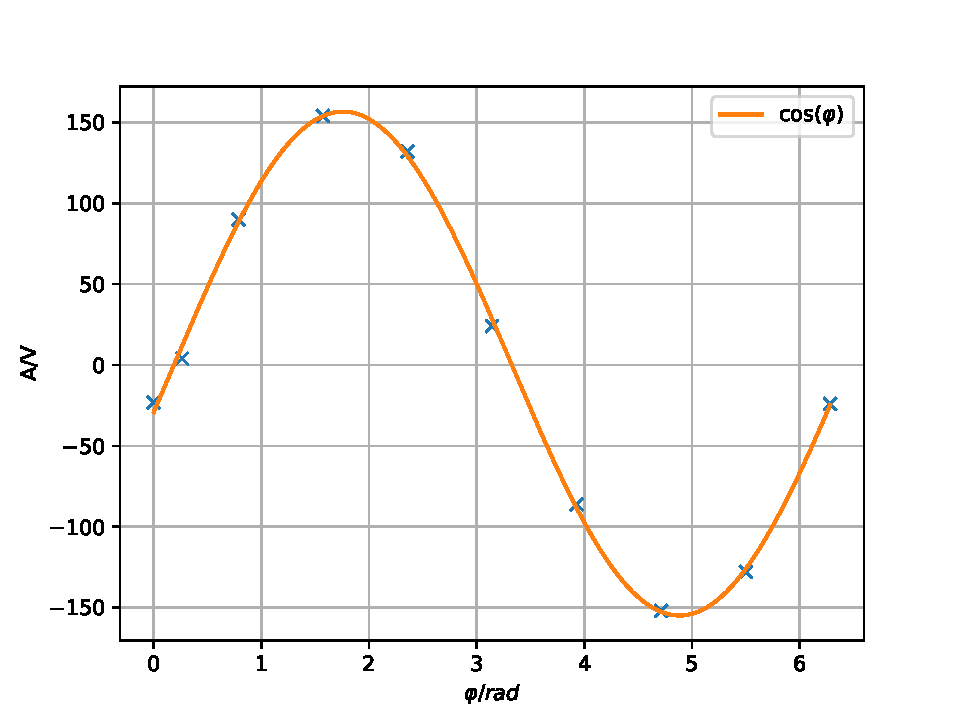
\includegraphics[width=\textwidth]{rausch.pdf}
  \caption{Phasenverschiebung $\varphi$ gegen Spannungsamplitude $A$ bei zugeschaltetem Rauschen}
  \label{fig:rauschplot}
\end{figure}
\FloatBarrier
Gefittet ist analog zur ersten Messreihe eine $\cos$-Funktion nach Gleichung \eqref{eqn:uoutcos}:
\begin{equation*}
  A= a \cos{(bx+c)}+d.
\end{equation*}
Die Parameter ergeben sich mit Python 3.6.3 zu
\begin{align*}
  a &=& \SI{-155.843  \pm 2.400}{V} \\
  b &=& \SI{  -1.004  \pm 0.006}{}\\
  c &=& \SI{ -13.944  \pm 0.020}{} \\
  d &=& \SI{   0.864  \pm 1.584}{V}.  \\
\end{align*}
Nach Gleichung \eqref{eqn:uoutcos} entspricht $a=\frac{2 \overline{U_{0}}}{\pi}$:
\begin{equation*}
  \overline{U_{0}}=\SI{244.798}{V}.
\end{equation*}
\FloatBarrier
\subsection{Überprüfung der Rauschunterdrückung mit dem Photodetektor}
Die Intensität U und der Abstand x zwischen der Diode und dem Detektor sind in Tabelle \ref{tab:Intensität} und in Abbildung \ref{fig:Intensität} zu finden.
\\In der Abbildung \ref{fig:Intensität} wird die Funktion mit
\begin{equation*}
  U=a \frac{1}{x^2}+b
\end{equation*}
angenähert.
\begin{figure}[h!]
  \centering
  \includegraphics[width=\textwidth]{Intensität.pdf}
  \caption{Intensität}
  \label{fig:Intensität}
\end{figure}
\input{Intensität.tex}
\\Die Parameter der gefitteten Funktion lauten:
\begin{equation*}
  a= \SI{1510.245 \pm 39.012}{W cm^2}
\end{equation*}
\begin{equation*}
  b=\SI{0.325\pm 0.061}{W}
\end{equation*}
\\Der genaue, maximale Abstand kann nicht angegeben werden, da die Möglichkeiten der Messapparatur vollständig ausgeschöpft wurden.
Die Steigung im Graphen ist bei den letzten Messungen annähernd konstant, daher wird
\begin{equation*}
  x_{max}=\SI{132.5}{cm}
\end{equation*}
 mit der Intensität $U_{I}=\SI{0.160}{V}$ gewählt.
\FloatBarrier




%\[  1.51024506e+03   3.25246387e-01]
%[[  1.52189388e+03  -1.51876309e+00]
% [ -1.51876309e+00   3.75030758e-03]]

%[  3.25246387e-01   1.51024506e+03]
%[[  3.75030758e-03  -1.51876309e+00]
% [ -1.51876309e+00   1.52189388e+03]]
